\section{Überblick}

\begin{frame}{Architektur des Wortschatzes}
\onslide<+->
\begin{itemize}[<+->]
  \item Sinnrelationen zwischen Lexemen (Fortsetzung)
	\item	Wortfelder
	\item	Wortfamilien
\end{itemize}
 \end{frame}


\section[Sinnrelationen II]{Sinnrelationen zwischen Lexemen II}

\begin{frame}{Kontiguitätsrelationen}
\onslide<+->
bestehen zwischen Lexemen als Referenten
\begin{itemize}[<+->]
	\item		die in der Wirklichkeit miteinander zu tun haben
	\item		d.\,h. meist räumlich oder zeitlich überlappen
\end{itemize}
\onslide<+->
\Zeile
\begin{exe}
	\ex\label{ex:kontiguitaetsrelationen-001}
    \begin{xlist}
		\ex{\label{ex:kontiguitaetsrelationen-001a}		Fuß ― Bein}
		\onslide<+->
		\ex{\label{ex:kontiguitaetsrelationen-001b}		Klinke ― Tür}
		\onslide<+->
		\ex{\label{ex:kontiguitaetsrelationen-001c}		Tag ― Woche}
	\end{xlist}
\end{exe}
\end{frame}

\begin{frame}{Kontiguitätsrelationen}
\onslide<+->
Teil–Ganzes wichtigste lexikalische Kontiguitätsrelation
\begin{itemize}[<+->]
	\item		Lexem für Teil heißt Meronym
	\item		Lexem für Ganzes nennt man Holonym
\end{itemize}
\onslide<+->
\Zeile
\begin{exe}
	\ex\label{ex:kontiguitaetsrelationen-002}
    \begin{xlist}
		\ex{\label{ex:kontiguitaetsrelationen-002a}		Finger~\textsubscript{\gruen{Meronym}} ― Hand~\textsubscript{\alert{Holonym}}}
		\onslide<+->
		\ex{\label{ex:kontiguitaetsrelationen-002b}		Ast~\textsubscript{\gruen{Meronym}} ― Baum~\textsubscript{\alert{Holonym}}}
		\onslide<+->
		\ex{\label{ex:kontiguitaetsrelationen-002c}		Felge~\textsubscript{\gruen{Meronym}} ― Rad~\textsubscript{\alert{Holonym}}}
		\onslide<+->
		\ex{\label{ex:kontiguitaetsrelationen-002d}		Herbst~\textsubscript{\gruen{Meronym}} ― Jahr~\textsubscript{\alert{Holonym}}}
	\end{xlist}
\end{exe}
\end{frame}

\begin{frame}{Kontiguitätsrelationen}
\onslide<+->
vier zentrale Eigenschaften von Meronymie
\begin{enumerate}
	\item		räumliche Inklusion des Teils durch das Ganze
	\item		Konstanz der Verbindung von Teil und Ganzem
	\item		Konstanz der Unterscheidbarkeit von Teil und Ganzem
	\item		Unmittelbarkeit der Relation zwischen Teil und Ganzem
\end{enumerate}
\end{frame}

\begin{frame}{Kontiguitätsrelationen}
\onslide<+->
räumliche Inklusion des Teils durch das Ganze
\begin{itemize}[<+->]
	\item		d.\,h. Meronym-Referent kleiner als Holonym-Referent
\end{itemize}
\onslide<+->
\Zeile
denn
\begin{itemize}[<+->]
	\item		mit \textit{Hand}~\textsubscript{\alert{Holonym}} immer \textit{Finger}~\textsubscript{\gruen{Meronym}} miteingeschlossen
	\item		{[\ldots]}
\end{itemize}
\end{frame}

\begin{frame}{Kontiguitätsrelationen}
\onslide<+->
Konstanz der Verbindung von Teil und Ganzem
\begin{itemize}[<+->]
	\item		d.\,h. Meronym-Referent und Holonym-Referent fest verbunden
\end{itemize}
\onslide<+->
\Zeile
denn
\begin{itemize}[<+->]
	\item		\textit{Ast}~\textsubscript{\gruen{Meronym}} und \textit{Baum}~\textsubscript{\alert{Holonym}} bilden Einheit
	\item		{[\ldots]}
\end{itemize}
\end{frame}

\begin{frame}{Kontiguitätsrelationen}
\onslide<+->
Konstanz der Unterscheidbarkeit von Teil und Ganzem
\begin{itemize}[<+->]
	\item		d.\,h. Meronym-Referent eindeutig von Holonym-Referent abgrenzbar
\end{itemize}
\onslide<+->
\Zeile
denn
\begin{itemize}[<+->]
	\item		\textit{Fuß}~\textsubscript{\gruen{Meronym}} und \textit{Bein}~\textsubscript{\alert{Holonym}} lassen sich trotz Einheit als Teile voneinander unterscheiden
	\item		{[\ldots]}
\end{itemize}
\end{frame}

\begin{frame}{Kontiguitätsrelationen}
\onslide<+->
Unmittelbarkeit der Relation zwischen Teil und Ganzem
\begin{itemize}[<+->]
	\item		d.\,h. keine andere Teil–Ganzes-Relation zwischen Meronym-Referent und Holonym-Referent geschaltet
\end{itemize}
\onslide<+->
\Zeile
denn
\begin{itemize}[<+->]
	\item		\textit{Finger}~\textsubscript{\gruen{Meronym~1}} zwar Teil von \textit{Hand}~\textsubscript{\alert{Holonym~1}}
	\item		so wie \textit{Hand}~\textsubscript{\gruen{Meronym~2}} Teil von \textit{Arm}~\textsubscript{\alert{Holonym~2}}
	\item		aber \textit{Finger}~\textsubscript{\gruen{Meronym~1}} nicht als Teil von \textit{Arm}~\textsubscript{\alert{Holonym~2}} zu bezeichnen
	\item		{[\ldots]}
\end{itemize}
\end{frame}

\begin{frame}{Kontiguitätsrelationen}
\onslide<+->
erläuterte Meronymie-Eigenschaften werfen Fragen auf
\begin{itemize}[<+->]
	\item		Ist Meronymie überhaupt eine sprachlich relevante Beziehung?
	\item		Oder beschreiben die einzelnen Kriterien nicht eher Verhältnisse in der Welt?
\end{itemize}
\onslide<+->
\Zeile
hier Kriterium Unmittelbarkeit der Relation entscheidend
\begin{itemize}[<+->]
	\item		weil Akzeptabilität von meronymischen Ausdrücken davon abhängt
	\item		somit Argument zugunsten von Meronymie als sprachlicher Relation
\end{itemize}
\end{frame}

\begin{frame}{Kontiguitätsrelationen}
\onslide<+->
Meronymie prinzipiell auch zwischen Verben ansetzbar
\begin{itemize}[<+->]
	\item		aufgrund von zeitlicher Inklusion eines Ereignisses in einem anderen
	\item		d.\,h. bestimmte Vorgänge überlappen
	\item		Meronym-Vorgang dabei als Teilphase von Holonym-Vorgang
\end{itemize}
\onslide<+->
\Zeile
\begin{exe}
	\ex\label{ex:kontiguitaetsrelationen-003}
    \begin{xlist}
		\ex{\label{ex:kontiguitaetsrelationen-003a}		einschlafen~\textsubscript{\gruen{Meronym}} ― schlafen~\textsubscript{\alert{Holonym}}}
		\onslide<+->
		\ex{\label{ex:kontiguitaetsrelationen-003b}		verblühen~\textsubscript{\gruen{Meronym}} ― blühen~\textsubscript{\alert{Holonym}}}
	\end{xlist}
\end{exe}
\end{frame}

\begin{frame}{Kontrastrelationen}
\onslide<+->
beruhen auf Bedeutungsgegensatz zwischen Lexemen
\begin{itemize}[<+->]
	\item		in verschiedenen Ausprägungen
	\item		z.\,T. abhängig von Wortart
\end{itemize}
\onslide<+->
\Zeile
je nach Art der Kontrastierbarkeit fünf Subtypen:
\begin{enumerate}[<+->]
	\item		Inkompatibilität
	\item		Antonymie
	\item		Komplementarität
	\item		Konversivität
	\item		Reversivität
\end{enumerate}
\end{frame}

\begin{frame}{Inkompatibilität}
\onslide<+->
falls Lexeme auf derselben Abstraktionsebene unvereinbar
\begin{itemize}[<+->]
	\item		d.\,h. Inkompatibilität i.\,e.\,S. besteht zwischen Kohyponymen
	\item		weil mit einem Referenten Bezug auf mehrere Kohyponyme unmöglich
	\item		andere Fälle von semantischer Unvereinbarkeit trivial Phänomen
\end{itemize}
\onslide<+->
\Zeile
\begin{exe}
	\ex\label{ex:inkompatibilitaet-001}
    \begin{xlist}
		\ex{\label{ex:inkompatibilitaet-001a}		Peter und Maria sind nicht mit dem Auto~\textsubscript{\gruen{Kohyponym~1}} gefahren, sondern mit dem Zug~\textsubscript{\alert{Kohyponym~2}}\,.}
		\onslide<+->
		\ex{\label{ex:inkompatibilitaet-001b}		Das ist doch kein Hamster~\textsubscript{\gruen{Kohyponym~1}}\,! Das ist ein Meerschweinchen~\textsubscript{\alert{Kohyponym~2}}\,.}
		\onslide<+->
		\ex[\textsuperscript{?}]{\label{ex:inkompatibilitaet-001c}		Wir haben gestern kein Fahrrad~\textsubscript{\gruen{\cancel{Kohyponym~1}}} gekauft, sondern einen Liegestuhl~\textsubscript{\alert{\cancel{Kohyponym~2}}} gekauft.}
	\end{xlist}
\end{exe}
\end{frame}

\begin{frame}{Antonymie}
\onslide<+->
inkompatible Lexeme mit Übergangsbereich
\begin{itemize}[<+->]
	\item		betrifft v.\,a. Adjektive
	\item		Antonyme markieren Endpunkte einer Skala
\end{itemize}
\onslide<+->
\Zeile
\begin{exe}
	\ex\label{ex:antonymie-001}
    \begin{xlist}
		\ex{\label{ex:antonymie-001a}		gut~\textsubscript{\gruen{Antonym 1}} ― böse~\textsubscript{\alert{Antonym 2}}}
		\onslide<+->
		\ex{\label{ex:antonymie-001b}		schön~\textsubscript{\gruen{Antonym 1}} ― hässlich~\textsubscript{\alert{Antonym 2}}}
		\onslide<+->
		\ex{\label{ex:antonymie-001c}		hell~\textsubscript{\gruen{Antonym 1}} ― dunkel~\textsubscript{\alert{Antonym 2}}}
		\onslide<+->
		\ex{\label{ex:antonymie-001d}		früh~\textsubscript{\gruen{Antonym 1}} ― spät~\textsubscript{\alert{Antonym 2}}}
	\end{xlist}
\end{exe}
\end{frame}

\begin{frame}{Kontiguitätsrelationen}
\onslide<+->
Übergangsbereich zwischen Antonymen
\begin{itemize}[<+->]
	\item		zwar größtenteils unbezeichnet oder nur ungenau bezeichnet
	\item		aber durch Gradierbarkeit von Antonymen zu erschließen
\end{itemize}
\onslide<+->
\Zeile
\begin{exe}
	\ex\label{ex:antonymie-002}
    \begin{xlist}
		\ex{\label{ex:antonymie-002a}		warm~\textsubscript{\gruen{Antonym 1}} ― lauwarm~\textsubscript{Übergangsbereich} ― kalt~\textsubscript{\alert{Antonym 2}}}
		\onslide<+->
		\ex{\label{ex:antonymie-002b}		hell~\textsubscript{\gruen{Antonym 1}} ― Ø ― dunkel~\textsubscript{\alert{Antonym 2}}}
		\onslide<+->
		\ex{\label{ex:antonymie-002c}		gut~\textsubscript{\gruen{Antonym 1}} ― \textsuperscript{?}mittelmäßig ― böse~\textsubscript{\alert{Antonym 2}}}
	\end{xlist}
\end{exe}
\end{frame}

\begin{frame}{Komplementarität}
\onslide<+->
inkompatible Lexeme ohne Übergangsbereich
\begin{itemize}[<+->]
	\item		betrifft ausschließlich nicht steigerbare Adjektive
	\item		mit logischem Verhältnis Kontradiktion
\end{itemize}
\onslide<+->
\Zeile
\begin{exe}
	\ex\label{ex:komplementaritaet-001}
    \begin{xlist}
		\ex{\label{ex:komplementaritaet-001a}		behandelt ― unbehandelt}
		\onslide<+->
		\ex{\label{ex:komplementaritaet-001b}		verheiratet ― ledig}
		\onslide<+->
		\ex{\label{ex:komplementaritaet-001c}		tot ― lebendig}
	\end{xlist}
\end{exe}
\end{frame}

\begin{frame}{Konversivität}
\onslide<+->
bei je nach Perspektive gegensätzlichen Lexemen
\begin{itemize}[<+->]
	\item		durch Vertauschung der Argumentstellen erkennbar
\end{itemize}
\onslide<+->
\Zeile
\begin{exe}
	\ex\label{ex:konversivitaet-001}
    \begin{xlist}
		\ex{\label{ex:konversivitaet-001a}		kaufen ― verkaufen}
		\onslide<+->
		\ex{\label{ex:konversivitaet-001b}		Ehemann ― Ehefrau}
	\end{xlist}
\end{exe}
\end{frame}

\begin{frame}{Reversivität}
\onslide<+->
ereigniszentrierter Gegensatz zwischen Lexemen
\begin{itemize}[<+->]
	\item		betrifft deshalb v.\,a. Verben
	\item		umschreibt Zyklus sich abwechselnder Ereignisse
\end{itemize}
\onslide<+->
\Zeile
\begin{exe}
	\ex\label{ex:reversivitaet-001}
    \begin{xlist}
		\ex{\label{ex:reversivitaet-001a}		aufschließen ― zuschließen}
		\onslide<+->
		\ex{\label{ex:reversivitaet-001b}		einschalten ― ausschalten}
	\end{xlist}
\end{exe}
\end{frame}

\begin{frame}{Skalare Relationen}
\onslide<+->
bestimmte Lexempaare schwierig zu verorten
\begin{itemize}[<+->]
	\item		scheinen zwischen Hyponymie und Antonymie zu schwanken
	\item		einerseits Lexem~1 ausgeprägte Art von Lexem~2
	\item		andererseits existiert Übergangsbereich zwischen beiden
\end{itemize}
\onslide<+->
\Zeile
\begin{exe}
	\ex\label{ex:skalare.relationen-001}
    \begin{xlist}
		\ex{\label{ex:skalare.relationen-001a}		Der Unterschied ist nicht nur \gruen{klein}, sondern \alert{winzig}.}
		\onslide<+->
		\ex{\label{ex:skalare.relationen-001b}		Peter \gruen{lief} nicht bloß zurück, er \alert{rannte}.}
		\onslide<+->
		\ex{\label{ex:skalare.relationen-001c}		Das ist keine \gruen{Bitte}, sondern eine \alert{Aufforderung}\,!}
	\end{xlist}
\end{exe}
\end{frame}

\begin{frame}{Skalare Relationen}
\onslide<+->
Antonymie liegt aber nicht vor
\begin{itemize}[<+->]
	\item		da kein Gegensatz zwischen Lexem~1 und Lexem~2
	\item		weshalb auch keine Inkompatibilität zwischen ihnen
\end{itemize}
\onslide<+->
\Zeile
denn
\begin{itemize}[<+->]
	\item		wenn etwas \textit{riesig}~\textsubscript{\alert{Lexem~2}}\,, dann mindestens auch \textit{groß}~\textsubscript{\gruen{Lexem~1}}
	\item		aber nur weil etwas \textit{groß}~\textsubscript{\gruen{Lexem~1}}\,, nicht zwangsläufig auch \textit{riesig}~\textsubscript{\alert{Lexem~2}}
	\item		{[\ldots]}
\end{itemize}
\end{frame}

\begin{frame}{Skalare Relationen}
\onslide<+->
auch Hyponymie liegt nicht vor
\begin{itemize}[<+->]
	\item		weil Übergangsbereich zwischen Lexem~1 und Lexem~2
	\item		vom einen zum anderen durch Verstärkung oder Abschwächung
\end{itemize}
\onslide<+->
\Zeile
Relation zwischen Lexemen wie \textit{groß} ― \textit{riesig} u.\,Ä.
\begin{itemize}[<+->]
	\item		insofern am besten als skalar zu beschreiben
\end{itemize}
\end{frame}

\begin{frame}{Syntagmatische Relationen}
\onslide<+->
bestehen zwischen Lexemen einer Äußerungskette
\begin{itemize}[<+->]
	\item		insofern horizontale Wortbeziehungen
	\item		d.\,h. Einschränkungen in Kombinationsmöglichkeit von Lexemen
\end{itemize}
\onslide<+->
\Zeile
grammatische Relationen zwischen Lexemen
\begin{itemize}[<+->]
	\item		für Lexikologie dabei vollkommen belanglos
\end{itemize}
\end{frame}

\begin{frame}{Syntagmatische Relationen}
\onslide<+->
für Etablierung von Syntagmatizität
\begin{itemize}[<+->]
	\item		aber einzig rekurrente Lexemkombinationen wichtig
\end{itemize}
\onslide<+->
\Zeile
\begin{exe}
	\ex\label{ex:syntagmatische.relationen-001}
    \begin{xlist}
		\ex{\label{ex:syntagmatische.relationen-001a}		Beschwerde ― einlegen}
		\onslide<+->
		\ex{\label{ex:syntagmatische.relationen-001b}		Hund ― bellen}
		\onslide<+->
		\ex{\label{ex:syntagmatische.relationen-001c}		Blume ― blühen}
	\end{xlist}
\end{exe}
\end{frame}

\begin{frame}{Syntagmatische Relationen}
\onslide<+->
drei Subtypen unterscheidbar:
\begin{enumerate}[<+->]
	\item		Relationen im Text
	\item		„Wesenhafte Bedeutungsbeziehungen“
	\item		Kollokationen
\end{enumerate}
\end{frame}

\begin{frame}{Relationen im Text}
\onslide<+->
paradigmatische Relationen manifestieren sich auf syntagmatischer Ebene
\begin{itemize}[<+->]
	\item		deshalb oft von zentraler Bedeutung für Textgestaltung
	\item		bes. Hyponymie und Synonymie
	\item		aber z.\,T. auch skalare Relationen
\end{itemize}
\onslide<+->
\Zeile
\begin{exe}
	\ex{\label{ex:relationen.im.text-001}		Maria stellte ihren Sportwagen~\textsubscript{\gruen{Synonym}~/ \alert{Hyponym}}~in der Tiefgarage ab. Sie war nicht nur glücklich~\textsubscript{\orongsch{Skalar}}~mit ihrem Flitzer~\textsubscript{\gruen{Synonym}}~, sondern wirklich stolz~\textsubscript{\orongsch{Skalar}}~darauf, obwohl sie sich zum Einkaufen manchmal ein kleineres Auto~\textsubscript{\alert{Hyperonym}}~wünschte.}
\end{exe}
\end{frame}

\begin{frame}{„Wesenhafte Bedeutungsbeziehungen“}
\onslide<+->
erwartbares Miteinandervorkommen bestimmter Lexeme
\begin{itemize}[<+->]
	\item		anhand von lexikalischen Unverträglichkeiten abzulesen
	\item		dafür i.\,d.\,R. Verbsemantik entscheidend
\end{itemize}
\onslide<+->
\Zeile
\begin{exe}
	\ex\label{ex:wesenhafte.bedeutungsbeziehungen-001}
    \begin{xlist}
		\ex[\textsuperscript{?}]{\label{ex:wesenhafte.bedeutungsbeziehungen-001a}		Er \gruen{log} \alert{aufrichtig}.}
		\onslide<+->
		\ex[\textsuperscript{?}]{\label{ex:wesenhafte.bedeutungsbeziehungen-001b}		Sie \gruen{schlief} \alert{munter}.}
		\onslide<+->
		\ex[\textsuperscript{?}]{\label{ex:wesenhafte.bedeutungsbeziehungen-001c}		Meine \alert{Krawatte} \gruen{redet}.}
		\onslide<+->
		\ex[\textsuperscript{?}]{\label{ex:wesenhafte.bedeutungsbeziehungen-001d}		Die \alert{Katze} \gruen{bellt} heute.}
	\end{xlist}
\end{exe}
\end{frame}

\begin{frame}{„Wesenhafte Bedeutungsbeziehungen“}
\onslide<+->
bestimmten Selektionsrestriktionen unterworfen
\begin{itemize}[<+->]
	\item		vom jeweiligen Verb vorgegeben
	\item		resultiert in semantischer Kongruenz
\end{itemize}
\onslide<+->
\Zeile
\begin{exe}
	\ex\label{ex:wesenhafte.bedeutungsbeziehungen-002}
    \begin{xlist}
		\ex{\label{ex:wesenhafte.bedeutungsbeziehungen-002a}		Die \gruen{Frau}~/ der \gruen{Junge} \gruen{liest} ein Buch.}
		\onslide<+->
		\ex[*]{\label{ex:wesenhafte.bedeutungsbeziehungen-002b}		Der \alert{Säugling}~/ das \alert{Auto}~/ der \alert{Hund} \gruen{liest} ein Buch.}
	\end{xlist}
	\onslide<+->
	\ex\label{ex:wesenhafte.bedeutungsbeziehungen-003}
    \begin{xlist}
		\ex{\label{ex:wesenhafte.bedeutungsbeziehungen-003a}		Peter \gruen{liest} ein \gruen{Buch}~/ einen \gruen{Roman}~/ ein \gruen{Plakat}.}
		\onslide<+->
		\ex[*]{\label{ex:wesenhafte.bedeutungsbeziehungen-003b}		Peter \gruen{liest} ein \alert{Auto}~/ einen \alert{Stuhl}~/ eine \alert{Lampe}.}
	\end{xlist}
\end{exe}
\end{frame}

\begin{frame}{„Wesenhafte Bedeutungsbeziehungen“}
\onslide<+->
zeigen sich z.\,T. aber nicht oder nur u.\,U. in syntagmatischer Verkettung
\begin{itemize}[<+->]
	\item		da bedingt durch Voraussetzungsrelation zwischen Lexemen
	\item		sodass Auslassung des vom Verb inhärent vorausgesetzten Substantivs üblich
	\item		außer nähere Bestimmung von Verbalhandlung mithilfe dessen intendiert
\end{itemize}
\onslide<+->
\Zeile
\begin{exe}
	\ex\label{ex:wesenhafte.bedeutungsbeziehungen-004}
    \begin{xlist}
		\ex[\textsuperscript{?}]{\label{ex:wesenhafte.bedeutungsbeziehungen-004a}		Sie \gruen{greift} mit der \alert{Hand} nach dem Brief.}
		\onslide<+->
		\ex{\label{ex:wesenhafte.bedeutungsbeziehungen-004b}		Sie \gruen{greift} mit zitternder \gruen{Hand} nach dem Brief.}
	\end{xlist}
	\onslide<+->
	\ex\label{ex:wesenhafte.bedeutungsbeziehungen-005}
    \begin{xlist}
		\ex[\textsuperscript{?}]{\label{ex:wesenhafte.bedeutungsbeziehungen-005a}		Er hat das Spiel mit den \alert{Augen} \gruen{gesehen}.}
		\onslide<+->
		\ex{\label{ex:wesenhafte.bedeutungsbeziehungen-005b}		Er hat das Spiel mit eigenen \gruen{Augen} \gruen{gesehen}.}
	\end{xlist}
\end{exe}
\end{frame}

\begin{frame}{„Wesenhafte Bedeutungsbeziehungen“}
\onslide<+->
wenn semantische Kongruenz bes. eng
\begin{itemize}[<+->]
	\item		entstehen häufig feste Lexempaare
	\item		nur bedingt veränderbar durch Ersetzung des Verbs
	\item		obwohl weniger restriktive Verben als Synonyme vorhanden
\end{itemize}
\onslide<+->
\Zeile
\begin{exe}
	\ex\label{ex:wesenhafte.bedeutungsbeziehungen-006}
    \begin{xlist}
		\ex{\label{ex:wesenhafte.bedeutungsbeziehungen-006a}		ein \gruen{Armband} \gruen{anlegen}~/ \alert{anziehen}}
		\onslide<+->
		\ex{\label{ex:wesenhafte.bedeutungsbeziehungen-006b}		einen \gruen{Ring} \gruen{anstecken}~/ \alert{anziehen}}
		\onslide<+->
		\ex{\label{ex:wesenhafte.bedeutungsbeziehungen-006c}		eine \gruen{Krawatte} \gruen{umbinden}~/ \alert{anziehen}}
		\onslide<+->
		\ex{\label{ex:wesenhafte.bedeutungsbeziehungen-006d}		einen \gruen{Hut} \gruen{aufsetzen}~/ \alert{anziehen}}
	\end{xlist}
\end{exe}
\end{frame}

\begin{frame}{„Wesenhafte Bedeutungsbeziehungen“}
\onslide<+->
Lesart eines Lexems oft durch syntagmatischen Kontext bestimmt
\begin{itemize}[<+->]
	\item		v.\,a. bei Adjektiven feststellbar
\end{itemize}
\onslide<+->
\Zeile
\begin{exe}
	\ex{\label{ex:wesenhafte.bedeutungsbeziehungen-007}		\gruen{rote} Rosen~: (natur)\gruen{rote} Haare~\textsubscript{[Nuancierung]}}
	\onslide<+->
	\ex{\label{ex:wesenhafte.bedeutungsbeziehungen-008}		\gruen{rotes} Pulver~: \gruen{rotes} Auto~\textsubscript{[Geltungsbereich]}}
\end{exe}
\end{frame}

\begin{frame}{Kollokationen}
\onslide<+->
bes. enge Wortverbindungen
\begin{itemize}[<+->]
	\item		insofern usuell und erwartbar
	\item		aber nicht „wesenhaft“
\end{itemize}
\onslide<+->
\Zeile
\begin{exe}
	\ex\label{ex:kollokationen-001}
    \begin{xlist}
		\ex{\label{ex:kollokationen-001a}		eingefleischter Junggeselle}
		\onslide<+->
		\ex{\label{ex:kollokationen-001b}		Geld abheben}
		\onslide<+->
		\ex{\label{ex:kollokationen-001c}		in Strömen regnen}
	\end{xlist}
\end{exe}
\end{frame}

\begin{frame}{Kollokationen}
\onslide<+->
spezifische Relation zwischen Bestandteilen
\begin{itemize}[<+->]
	\item		Lexem im Zentrum heißt Basis
	\item		satellitenhaftes Lexem nennt man Kollokator
\end{itemize}
\onslide<+->
\Zeile
\begin{exe}
	\ex\label{ex:kollokationen-002}
    \begin{xlist}
		\ex{\label{ex:kollokationen-002a}		eingefleischter~\textsubscript{\alert{Kollokator}} Junggeselle~\textsubscript{\gruen{Basis}}}
		\onslide<+->
		\ex{\label{ex:kollokationen-002b}		Geld~\textsubscript{\gruen{Basis}} abheben~\textsubscript{\alert{Kollokator}}}
		\onslide<+->
		\ex{\label{ex:kollokationen-002c}		in Strömen~\textsubscript{\alert{Kollokator}} regnen~\textsubscript{\gruen{Basis}}}
	\end{xlist}
\end{exe}
\end{frame}

\begin{frame}{Kollokationen}
\onslide<+->
zeichnen sich durch gesteigerte Akzeptabilität aus
\begin{itemize}[<+->]
	\item		i.\,d.\,R. allgemein bevorzugter Ausdruck für Sachverhalt
	\item		Kollokator deshalb nur bedingt durch Synonyme ersetzbar
\end{itemize}
\onslide<+->
\Zeile
\begin{exe}
	\ex\label{ex:kollokationen-003}
    \begin{xlist}
		\ex{\label{ex:kollokationen-003a}		\gruen{frisch}~/ \alert{jüngst} gestrichen}
		\onslide<+->
		\ex{\label{ex:kollokationen-003b}		\gruen{harsche}~/ \alert{raue} Kritik \gruen{üben}~/ \alert{äußern}}
		\onslide<+->
		\ex{\label{ex:kollokationen-003c}		der Zorn \gruen{verraucht}~/ \gruen{verfliegt}}
	\end{xlist}
\end{exe}
\end{frame}

\begin{frame}{Kollokationen}
\onslide<+->
als transparente Wortverbindungen
\begin{itemize}[<+->]
	\item		bei denen Basis Lesart von Kollokation festlegt
	\item		d.\,h. nicht idiomatisch
\end{itemize}
\onslide<+->
\Zeile
\begin{exe}
	\ex{\label{ex:kollokationen-004}		frische~\textsubscript{\alert{Kollokator} ‚unverbraucht‘} Kräfte~\textsubscript{\gruen{Basis}}~: frischer~\textsubscript{\alert{Kollokator} ‚kühl‘} Wind~\textsubscript{\gruen{Basis}}}
\end{exe}
\end{frame}

\begin{frame}{Kollokationen}{Sonderfall statistische Kookkurrenzen}
\onslide<+->
rein statistischer Kollokationsbegriff
\begin{itemize}[<+->]
	\item		ergibt sich aus Frequenz von Wortverbindungen
	\item		innerhalb eines bestimmten Korpus
\end{itemize}
\onslide<+->
\Zeile
obwohl nicht aufgrund von Grammatik definiert
\begin{itemize}[<+->]
	\item		umfassen Kookkurenzen auch linguistisch relevante Kategorien
\end{itemize}
\end{frame}

\begin{frame}{Kollokationen}{Sonderfall statistische Kookkurrenzen}
\center
\begin{figure}
\includegraphics[width=0.95\textwidth]{\GRAPHPATH/DWDS_Wortwolke-Wort}
%\includegraphics[width=0.95\textwidth]{DWDS_Wortwolke-Wort}
\caption{Wortwolke für das Lexem \textit{Wort} (DWDS Wortprofil)}
\end{figure}
\end{frame}

\section{Wortfelder}

\section{Wortfamilien}
